\section{Characterization Problem Results}
\label{sec:CharResults}

To quantify the $\Omega$-method success for a variety of anisotropy-inducing
physics, we will present various forms of the Figure of Merit, as described in
Section \ref{sec:successmetrics}.
In the preceding subsections, a
subset of flux anisotropy-inducing physics have been identified
and a subset of problems that contain these physics have been conceived.
In this section, the results for CADIS-$\Omega$, CADIS, and nonbiased Monte Carlo
will be presented for each of these problems. Explanations on the performance of
the $\Omega$ methods will accompany the results for each problem. In some cases,
variants of problems were run to confirm or refute observations seen
in other problems.

\subsection{Computational Specifications}
\label{subsec:comp_specs}

As noted in a number of the previous sections, hybrid methods require both a
deterministic and a Monte Carlo calculation to obtain a problem result. These
transport codes require different computational parameters to obtain an answer.
For the characterization problems the computational parameters are summarized in
Table \ref{tab:simulation_defaults}; the parameters for the deterministic and
Monte Carlo calculations are demarcated in the table.

\begin{table}[h!]
  \centering
  \begin{tabular}{l|m{5cm}}
\toprule
Parameter Type & Parameter Value \\
\midrule \midrule
\multicolumn{2}{c}{ADVANTG Values$^1$} \\
\midrule
P$_N$ Order               &    $3$ \\
Quadrature Type           &  Quadruple Range \\
Quadrature Order          &    $10$ \\
Spatial Solver            &  Step Characteristic \\
Energy Group Library$^{\dagger}$     &    27G19N \\
Boundary Conditions & vacuum \\
\midrule \midrule
\multicolumn{2}{c}{MCNP Values$^2$} \\
\midrule
Particle Count      &   $1e7$ \\
Boundary Conditions & vacuum \\
\bottomrule
\end{tabular}
\begin{flushleft}
\footnotesize{
  $^1$ ADVANTG runs of the characterization problems
  were run on 16 cores of a 32 core node, with 256Gb of memory on
  an Oak Ridge National Laboratory compute cluster maintained by the Radiation
  Transport and Nuclear Systems Division. \\
  $^2$ MCNP runs of the characterization problems were run on the same
 machine, with 256Gb of memory but using all 32 cores of the node. \\
  $^{\dagger}$ Parameter type that has no default in ADVANTG.}
\end{flushleft}


  \caption[Default simulation values for characterization problems.]{
    Default simulation values for the characterization problems. The values for
    ADVANTG primarily signify parameters used to run Denovo, with exceptions for
    calculating biasing parameters, which is done exclusively in ADVANTG.
    MCNP-specific values are those used for Monte Carlo runs.
  }
  \label{tab:simulation_defaults}
\end{table}

The first portion of the table summarizes the values used by ADVANTG. Note that
these values all pertain to the Denovo deterministic solver, which is set up by
ADVANTG. The parameter types marked with a dagger have no default in ADVANTG.
We have chosen to use a relatively course 27 group energy group library.
Because the characterization problems are meant to identify the method's
performance pertaining to flux anisotropy, and we expect the energy group
structure to have less of an effect on anisotropy conditions than other
parameters, we opted for a
computationally inexpensive energy group mesh for the deterministic solver.
Further, this group library was designed for radiation shielding applications,
so it applies to the majority of the characterization problems.

The boundary conditions for all of the characterization problems will be vacuum.
At this time, ADVANTG does not support reflective or mirror boundary conditions
so this is a limitation in application space that we cannot address at this
time. The Monte Carlo code we use does support vacuum boundary conditions, but a
discrepancy in boundary conditions between deterministic and Monte Carlo
calculations would result in the simulation of a fundamentally different problem.

Unless noted, the values in this subsection of the table are ADVANTG
default values. They are a good initial choice for characterization of the
method because they are often chosen as the parameters for hybrid methods studies
by experienced and inexperienced ADAVANTG users.
Further, these values are defaults in ADVANTG for their
computational stability, such as not having negative valued weights or fluxes,
stable convergence, a relatively fast time to a solution, et cetera. Due to
the good properties exhibited by the solver options and because users first
using the $\Omega$-methods are likely to choose these values, the values in
Table \ref{tab:simulation_defaults} will be used for the characterization of the
$\Omega$-methods.

The latter section of the table summarizes the Monte Carlo code MCNP values for
each of the problems. The value of $1e7$ particles as a particle cutoff
was chosen because it made the
error bins in the majority of the nonbiased Monte Carlo
characterization problems less than 100\%. In some problems that are
extraordinarily difficult for Monte Carlo to solve without biasing, there were
tally bins with very high errors. In the following subsections they will be
clearly indicated and their results will not be plotted so as to not obfuscate
the CADIS and CADIS-$\Omega$ results. Time cutoffs were not chosen because
we decided to measure how effective the $\Omega$ methods were at reducing the
variance per particle. Depending on the flux maps generated from CADIS and
CADIS-$\Omega$, the time to transport a finite amount of particles may vary. As
a result, the reported times from a simulation can tell us whether the method
requires more sampling than other methods in addition to how fast it takes to
reach a desired relative error.

The responses in the NaI detectors of each of
the problems was measured with an MCNP track length tally (f4). The tally was
energetically binned to match the dataset of the multigroup dataset provided in
ADVANTG, and the entire volume of the detectors were used with no spatial
binning. It should be noted that while the tally is energetically binned, Monte
Carlo transport is not discretized in space or energy like deterministic
transport. In a nonbiased analog Monte Carlo calculation, transport is
completely continuous in space, energy, and angle. In a hybrid calculation using
VR parameters from a deterministic solution, the VR parameters will be
discretized to reflect the solution obtained from the determinstic solver. As a
result, the particle's transit throughout the
problem will be a combination of sampling both continuous and discretized-energy
dependent factors. Consider a particle that goes through a scattering event
in shielding material. In this scattering event, the particle samples from a
continuous-energy cross section and changes direction based on its energy.
However, depending on how much energy it loses in the scattering event it may
cross into the energy range of a lower-energy weight window and will require
further sampling.

All characterization problems were run on Remus, a machine operated and
maintained by the Radiation Transport and Nuclear Systems Division at Oak Ridge
National Laboratory. The ADVANTG runs were run on 16 cores of a 32 core node,
with 256Gb of memory. The MCNP runs were run on the same machine, with 256Gb of
memory but using all 32 cores of the node.

Each problem presented in Section \ref{sec:CharResults} will
use the values specified in Table \ref{tab:simulation_defaults}
unless otherwise noted.
Times to transport the Monte Carlo particle quantity varies between methods
due to differences in sampling. Monte Carlo and ADVANTG
inputs and directions on how to acquire them are
provided in Appendix \ref{sec:github_codes}.

\subsection{Single Turn Labyrinth}
\label{subsec:maze2}

The analysis of the characterization problems begins with the single turn
labyrinth.
The single turn labyrinth FOM results are summarized in Table \ref{tab:maze2foms},
and are illustrated in Figures \ref{fig:maze2result} and \ref{fig:maze2error}.
The table has six FOM values for CADIS and CADIS-$\Omega$ results, and three FOM
values for the analog (nonbiased) Monte Carlo results. The equations to
calculate each of these FOMS is summarized in Table \ref{tab:fom_defaults}.

\begin{table}[h!]
  \centering
  \begin{tabular}{lrrrrr}
\toprule
{} & \multicolumn{2}{c}{CADIS}   & \multicolumn{2}{c}{CADIS-$\Omega$}  & analog \\
{} &    MC & MC$_{hybrid}$ &         MC & MC$_{hybrid}$ &     MC \\
\midrule
tally avg   &  18.6 &        14.9 &       2.36 &        1.56 &   17.4 \\
max RE      &  2.76 &        2.21 &      0.481 &       0.318 & 0.0857 \\
min RE      &   249 &         200 &        196 &         130 &    -- \\
time (mins) &  67.7 &        84.4 &        157 &         237 &   11.7 \\
\bottomrule
\end{tabular}

  \caption[Figure of Merit comparison for single turn maze.]{Figure of Merit
    comparison for single turn maze.
    The relative errors used are the tally average relative error, the tally maximum relative
  error, and the tally minimum relative error; the times are total walltimes for
  the Monte Carlo calculation and the sum of the hybrid method software, the
  deterministic transport time, and the Monte Carlo calculation time.}
  \label{tab:maze2foms}
\end{table}

\begin{table}[h!]
  \centering
  \begin{tabular}{llrrr}
\toprule
          &              &          cadis &     cadisangle &         analog \\
          &              & time (minutes) & time (minutes) & time (minutes) \\
\midrule
MCNP time & total &          67.71 &         157.01 &          11.67 \\
deterministic time & advantg\_time &           0.26 &           0.28 &            -- \\
          & denovo\_time &          16.41 &          78.19 &            -- \\
          & dispose\_time &           0.01 &           0.40 &            -- \\
          & omega\_time &           0.00 &           1.61 &            -- \\
          & total &          16.67 &          80.08 &            -- \\
wall time &              &          84.38 &         237.09 &          11.67 \\
\bottomrule
\end{tabular}

  \caption[Detailed timing results for single turn maze.]
  {Detailed timing results for single turn maze.}
  \label{tab:maze2times}
\end{table}

In Table \ref{tab:maze2foms} the FOM results for CADIS, CADIS-$\Omega$, and
nonbiased Monte Carlo for the single turn maze are presented. In all cases, the
CADIS FOMs are better than those obtained by CADIS-$\Omega$. The FOMS
calculated using the tally average relative error are better in the nonbiased
analog Monte Carlo than CADIS-$\Omega$ as well. However, this is a product of
two effects: the time for the analog to run the same particle count is far
shorter than either CADIS or CADIS-$\Omega$. As a result, to obtain the same
FOM, CADIS-$\Omega$ needs to have $R_1/R_2 = \sqrt{T_2/T_1}$ (this is from
taking a ratio of the FOMs) the tally average
relative error, or ~$0.27$. Because this problem is highly scattering and many
low-energy particles can make it through the concrete labyrinth, even the analog
can have good sampling at low energies, resulting in a tally average FOM that
reaches this threshold.

Table \ref{tab:maze2times} contains more detailed timing information spent in
each of the codes for each type of problem. We can see that the Monte Carlo
runtime for CADIS-$\Omega$ is more than twice that of CADIS, and almost fifteen
times that of the nonbiased analog Monte Carlo. The time to run just the
hybrid/deterministic portion of the calculation is also four times longer for
CADIS-$\Omega$ than it is for CADIS. These disparities in runtimes have a strong
negative impact on the CADIS-$\Omega$ FOMs, which was observed in the FOM
results in Table \ref{tab:maze2foms}.

\begin{figure}[h!]
  \centering
  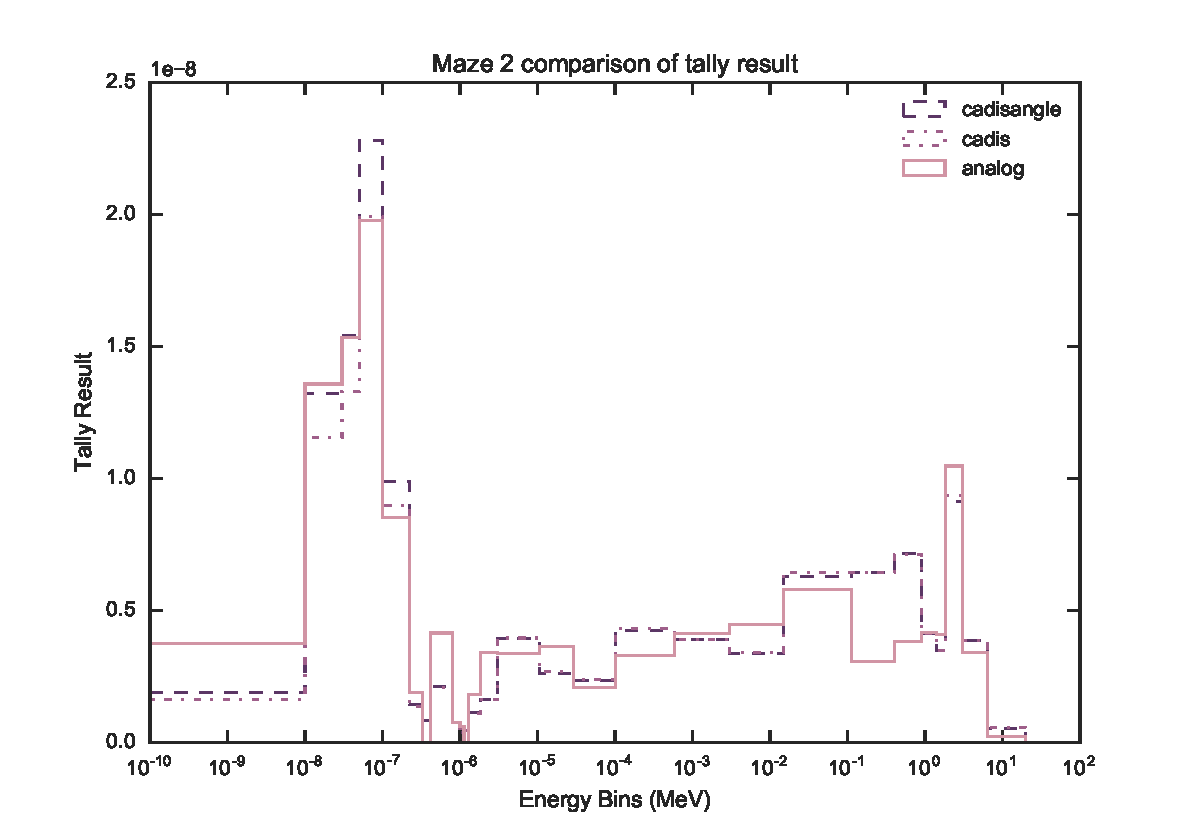
\includegraphics[height=10cm]{./chapters/characterization_probs/figures/char/maze2/maze_2_tally_result_compare.pdf}
  \caption[Tally results comparison between methods for single turn labyrinth.]
  {Tally results comparison between methods for single turn labyrinth.}
  \label{fig:maze2result}
\end{figure}

\begin{figure}[h!]
  \centering
  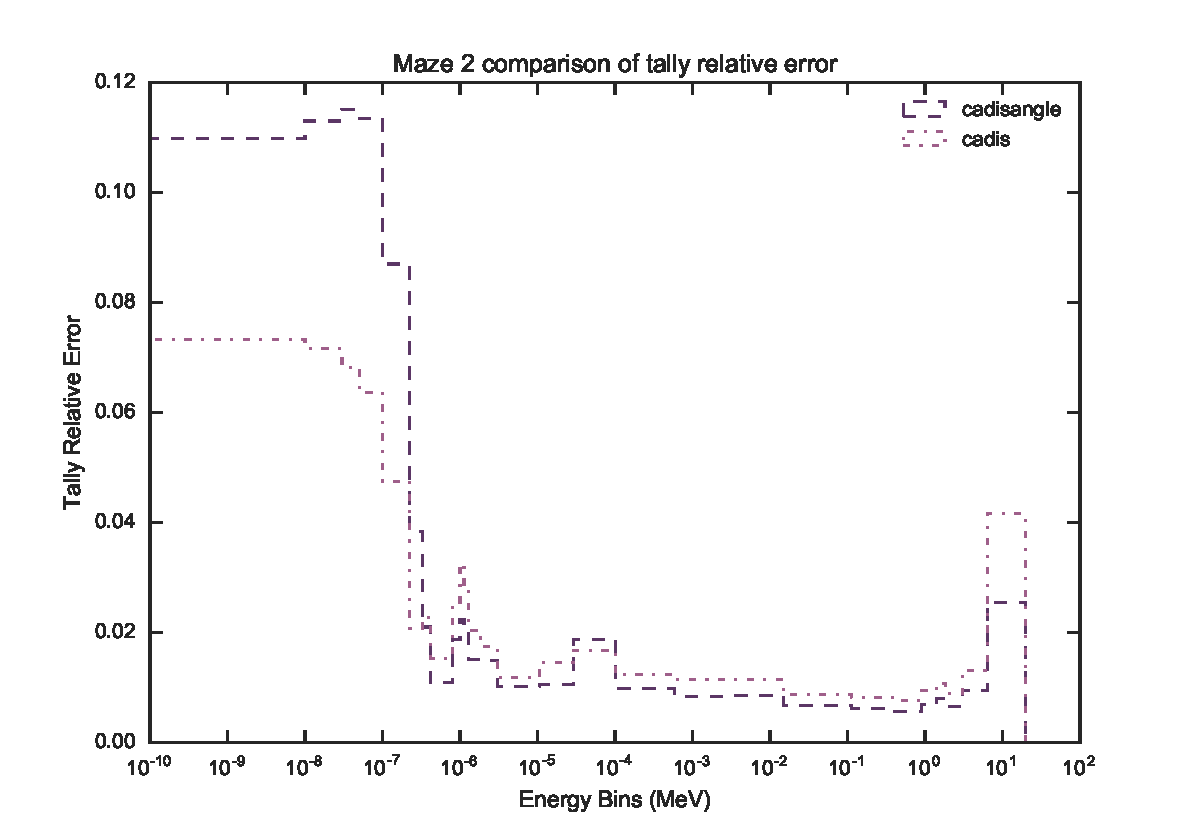
\includegraphics[height=10cm]{./chapters/characterization_probs/figures/char/maze2/maze_2_tally_error_compare.pdf}
  \caption[Tally relative error comparison between methods for single turn
  labyrinth]{Tally relative error comparison between methods for a single turn
  labyrinth.}
  \label{fig:maze2error}
\end{figure}

Figures \ref{fig:maze2result} and \ref{fig:maze2error} show the tally result and
the relative errors for each result in the single turn maze, respectively.
This particular relative error plot,
Figure \ref{fig:maze2error}, does not include the
relative error bins of the analog result because they are significantly higher
than the CADIS and CADIS-$\Omega$ results. This is further confirmed in Table
\ref{tab:maze2foms}, where the minimum relative error FOM is a non-tallied bin.

By inspecting Figure \ref{fig:maze2result}, one can observe that the CADIS and
CADIS-$\Omega$ results are in agreement in bins greater that $10^{-7}$ MeV. At
lower energy bins, CADIS-$\Omega$ generally has a higher value for the tally
result than standard CADIS. However, in comparing the errors for these low energy
bins in Figure $\ref{fig:maze2error}$, CADIS has a lower relative error. This
indicates that CADIS sampled many more low-weight particles than CADIS-$\Omega$
in these regions. Conversely, CADIS-$\Omega$ has a lower calculated relative
error than CADIS for bins greater than ~$5*10^{-6}$ MeV. This is expected, as
higher energy particles generally exhibit a stronger angular dependence than
low-energy particles. In geometric and energetic regions
where the angular dependence is stronger,
the importance map generated by CADIS-$\Omega$ may show more of an effect in
improving the relative error.

% High energy particles exiting the maze towards the tally
% detector have much longer mean free paths than the low energy particles, and
% will generally show a much stronger effect in the $\Omega$-flux in those
% regions. This is illustrated in Figure \ref{fig:}. The shape of the $\Omega$
% flux around the detector region is much more strongly dependent on direction in
% the high energy group 000 flux than it is for the lower energy group 026 flux.
% Despite having lower relative errors than CADIS at higher energies,
% CADIS-$\Omega$ has lower FOMs than CADIS for the FOMS calculated with the
% minimum relative error. As discussed previously, this is due to the long runtime
% of CADIS-$\Omega$, which is more than twice as long as CADIS. From this, we can
% conclude that while CADIS-$\Omega$ is better at transporting particles in high
% energy regions than CADIS, achieving lower relative errors, the length of time
% to do so is prohibitive and achievable by CADIS should the runtimes be the same
% for both.
%
% [todo: Omega flux lot of group 00]
%
% [todo: Omega flux plot of group 026]

\subsection{Multiple Turn Labyrinth}
\label{subsec:maze1}

The multiple turn labyrinth is built off of the single turn labyrinth geometry.
The labyrinth materials are much the same, but the geometry differs. Table
\ref{tab:maze1foms} summarizes the Figure of Merit results for CADIS,
CADIS-$\Omega$ and nonbiased Monte Carlo. Figures \ref{fig:maze1result} and
\ref{fig:maze1error} show the results obtained by the track length tally in each
method.

\begin{table}[h!]
  \centering
  \begin{tabular}{lrrrrr}
\toprule
{} & cadis &             & cadisangle &             & analog \\
{} &    MC & MC\_adjusted &         MC & MC\_adjusted &     MC \\
\midrule
tally avg   &   327 &         248 &        224 &          71 &  0.054 \\
max RE      &  1.46 &        1.11 &       1.02 &       0.322 & 0.0393 \\
min RE      &   113 &        85.6 &         71 &        22.5 &    -- \\
time (mins) &  51.5 &          68 &       35.5 &         112 &   25.5 \\
\bottomrule
\end{tabular}

  \caption[Figure of Merit comparison for multiple turn maze.]{Figure of Merit
    comparison for multiple turn maze.}
  \label{tab:maze1foms}
\end{table}

\begin{table}[h!]
  \centering
  \begin{tabular}{llrrr}
\toprule
          &              &          cadis &     cadisangle &         analog \\
          &              & time (minutes) & time (minutes) & time (minutes) \\
\midrule
MCNP time & total &          51.52 &          35.55 &          25.46 \\
deterministic time & advantg\_time &           0.25 &           0.21 &            -- \\
          & denovo\_time &          16.28 &          74.85 &            -- \\
          & dispose\_time &           0.01 &           0.40 &            -- \\
          & omega\_time &           0.00 &           1.74 &            -- \\
          & total &          16.53 &          76.80 &            -- \\
wall time &              &          68.05 &         112.35 &          25.46 \\
\bottomrule
\end{tabular}

  \caption[Detailed timing results for multiple turn maze.]
  {Detailed timing results for multiple turn maze.}
  \label{tab:maze1times}
\end{table}

In Tables \ref{tab:maze1foms} and \ref{tab:maze1times}
it is notable that the CADIS-$\Omega$ runtime is
shorter in the Monte Carlo simulation than CADIS. This differs most of the other
cases presented in this section. Both CADIS and CADIS-$\Omega$ outperform the
analog by a factor of $10^2$ or $10^3$, indicating the necessity of variance
reduction for a problem like this. In comparing the FOMs, CADIS slightly outperforms
CADIS-$\Omega$ for all relative errors, meaning that the time
to reach any relative error will be achieved faster by CADIS.

\begin{figure}[h!]
  \centering
  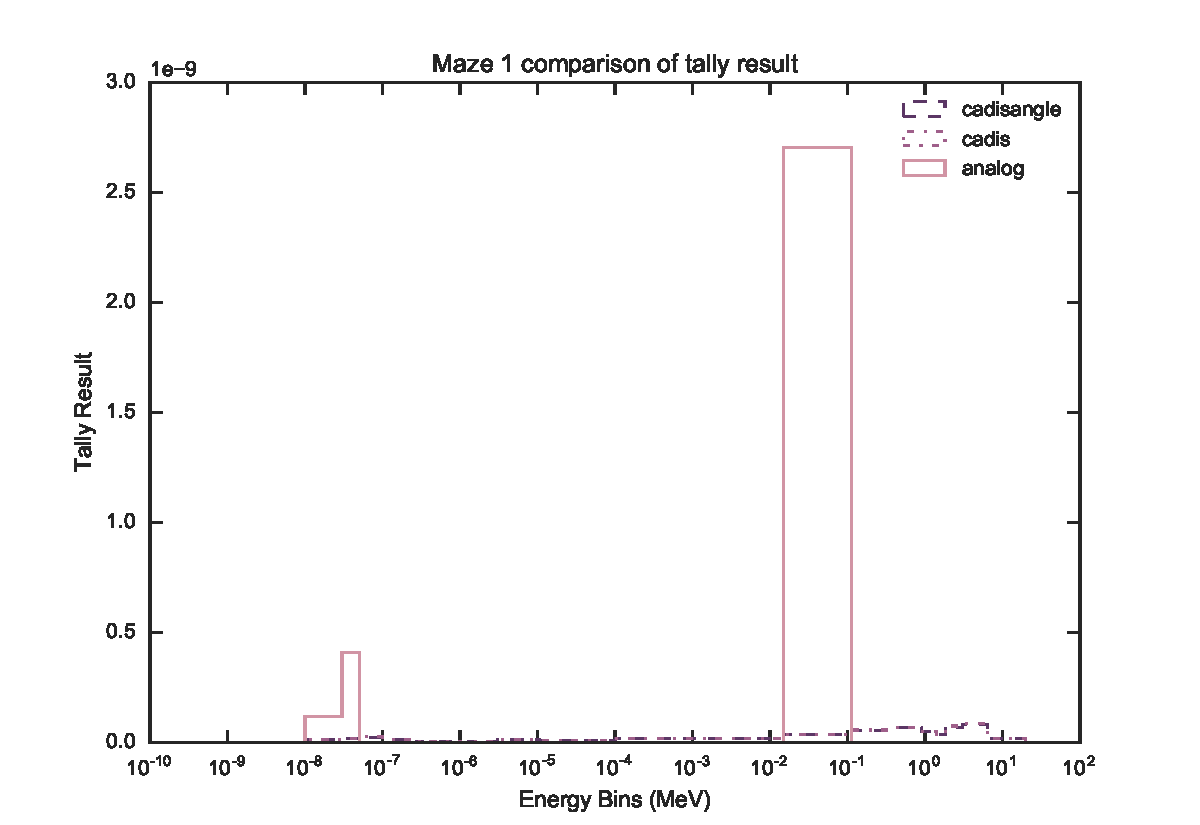
\includegraphics[height=10cm]{./chapters/characterization_probs/figures/char/maze1/maze_1_tally_result_compare.pdf}
  \caption[Tally results comparison between methods for multiple turn labyrinth.]
  {Tally results comparison between methods for multiple turn labyrinth. }
  \label{fig:maze1result}
\end{figure}

\begin{figure}[h!]
  \centering
  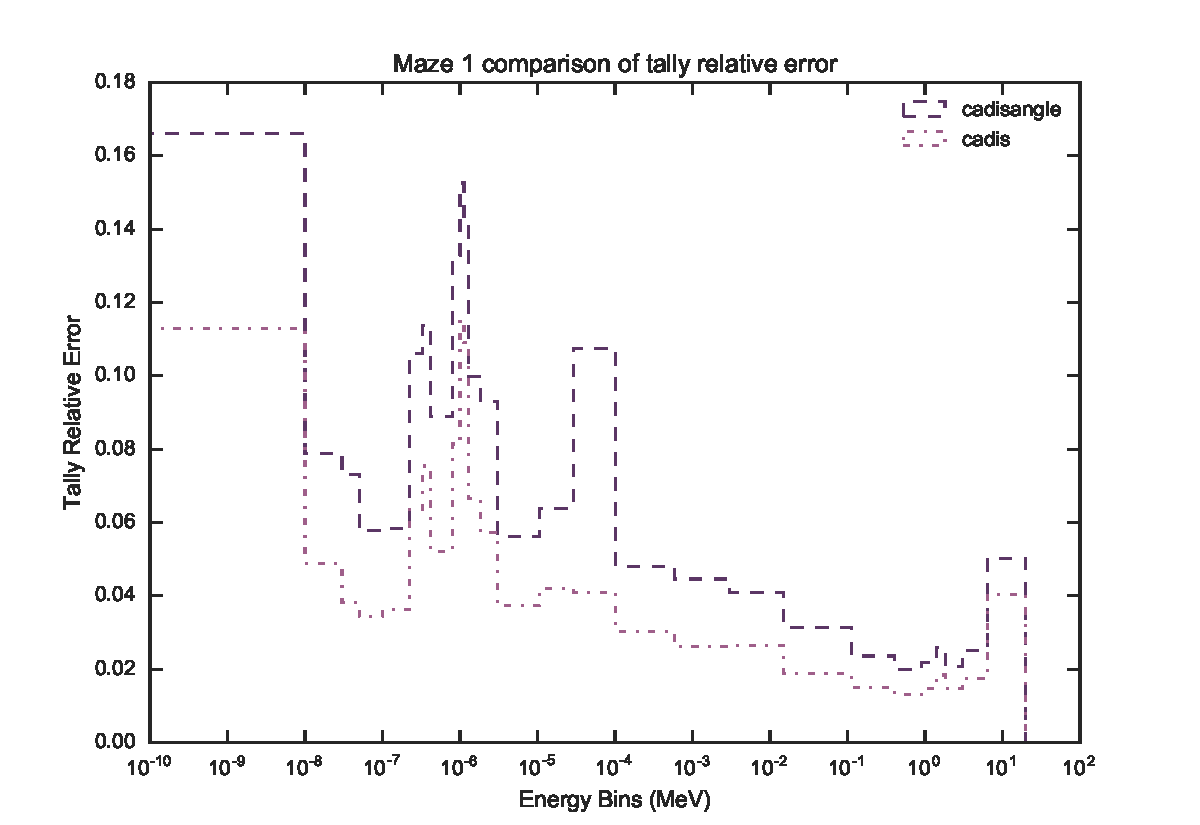
\includegraphics[height=10cm]{./chapters/characterization_probs/figures/char/maze1/maze_1_tally_error_compare.pdf}
  \caption[Tally relative error comparison between methods for multiple turn labyrinth]
  {Tally relative error comparison between methods for a multiple turn
  labyrinth. }
  \label{fig:maze1error}
\end{figure}

Looking at Figures \ref{fig:maze1result} and \ref{fig:maze1error}, we can see
that the analog Monte Carlo differ significantly from either CADIS or
CADIS-$\Omega$. Two distinct regions of tally bins have been recorded in the
analog case: a high energy region comprised of particles that have scattered
very few times before reaching the detector, and a much smaller low energy
region, comprised of particles that are very thermal. These thermal particles
have a very small MFP in the concrete labyrinth, thus the majority of them were
absorbed in the shield. However, given the errors on this result, these results are
not trustworthy. In the case of this problem, some of what was discussed in the
single-turn labyrinth is confirmed. This particular case requires that particles
scatter several more times if they are to exit the labyrinth from the air duct.
As a result, the spectrum is more thermal than the first case and the problem
has less anisotropy. As discussed in the single-turn labyrinth, CADIS
outperformed CADIS-$\Omega$ in problems in energy bins that had less angular
dependence. Because this problem has far more scattering event, it overall has
less angular dependence and CADIS outperforms CADIS-$\Omega$ in all energy bins.
This problem is poorly suited to CADIS-$\Omega$.

In Section \ref{subsec:maze2}, it was discussed that higher energy regions that
contribute to the tally are more anisotropic, and that these regions benefit
more from the $\Omega$-flux map than they do with standard CADIS' importance
map. First, looking at the metric three distributions for both the single- and
multiple-turn labyrinths in Figure \ref{fig:labyrinthviolins}, we can see shifts
up to much higher values for very isotropic energy groups.

\begin{figure}[htb!]
  \centering
  \begin{subfigure}[t]{\textwidth}
    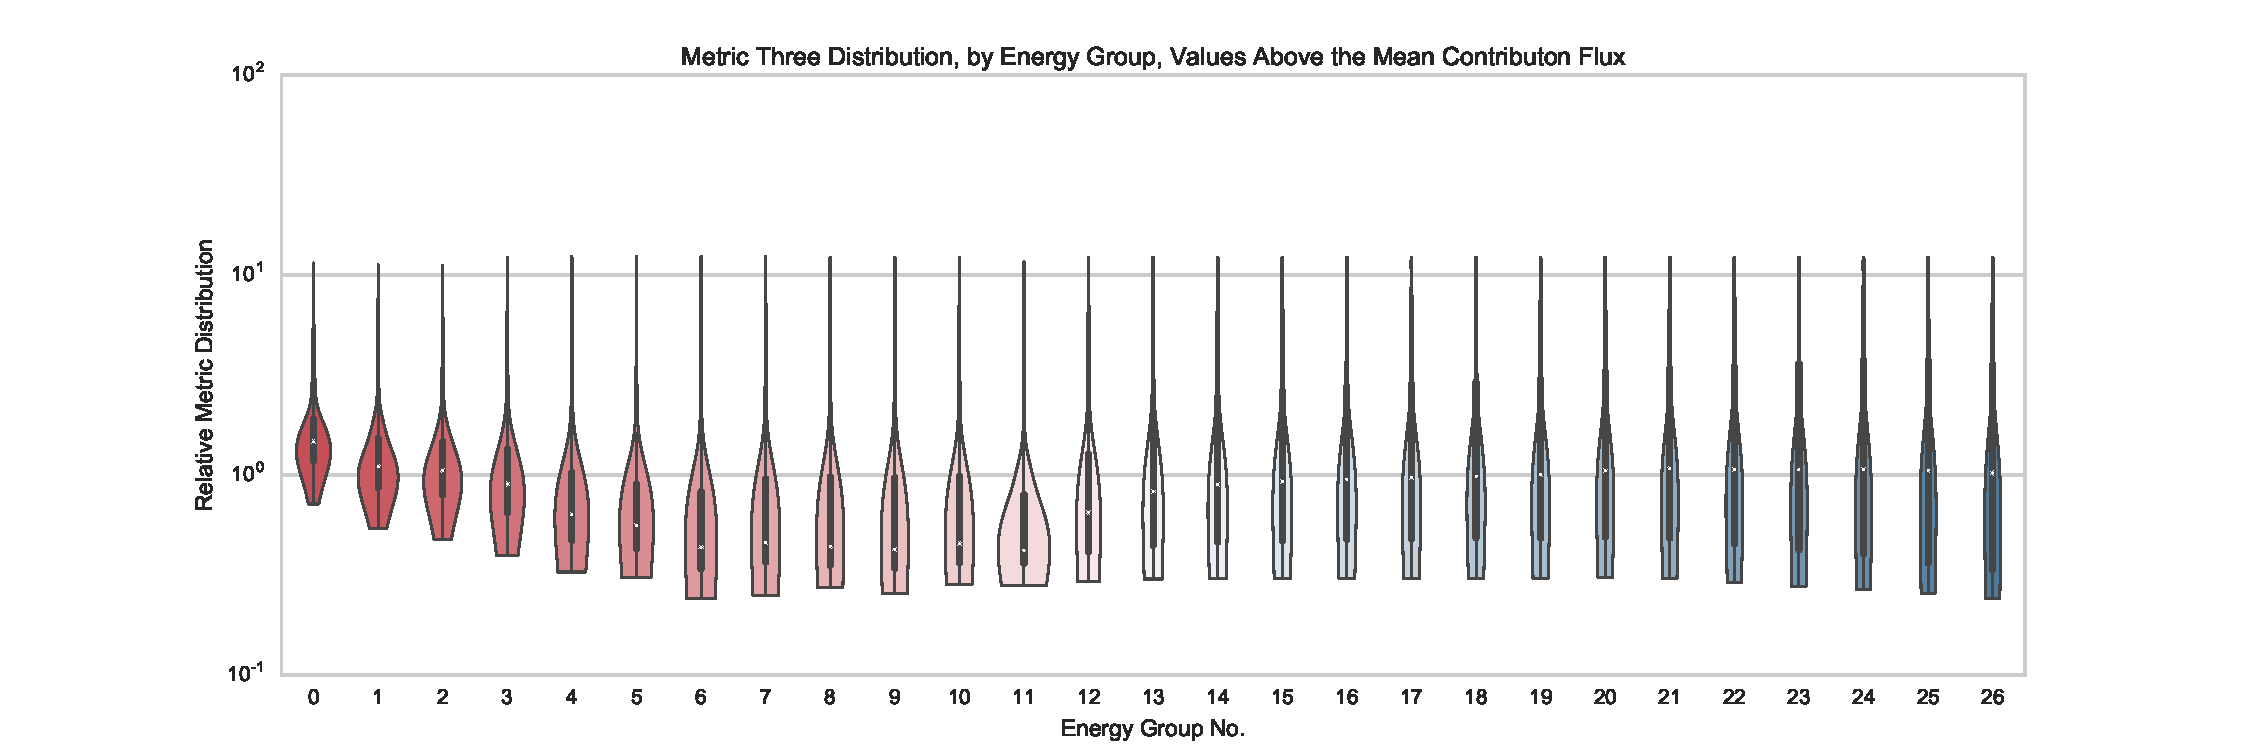
\includegraphics[width=\linewidth]{./chapters/characterization_probs/figures/char/maze2/metric_three_violin_mean.pdf}
    \caption{M$_{3}$ distribution for single turn labyrinth}
    \label{fig:maze2M3violins}
  \end{subfigure}
\end{figure}
\begin{figure}[htb!]\ContinuedFloat
  \centering
  \begin{subfigure}[t]{\textwidth}
    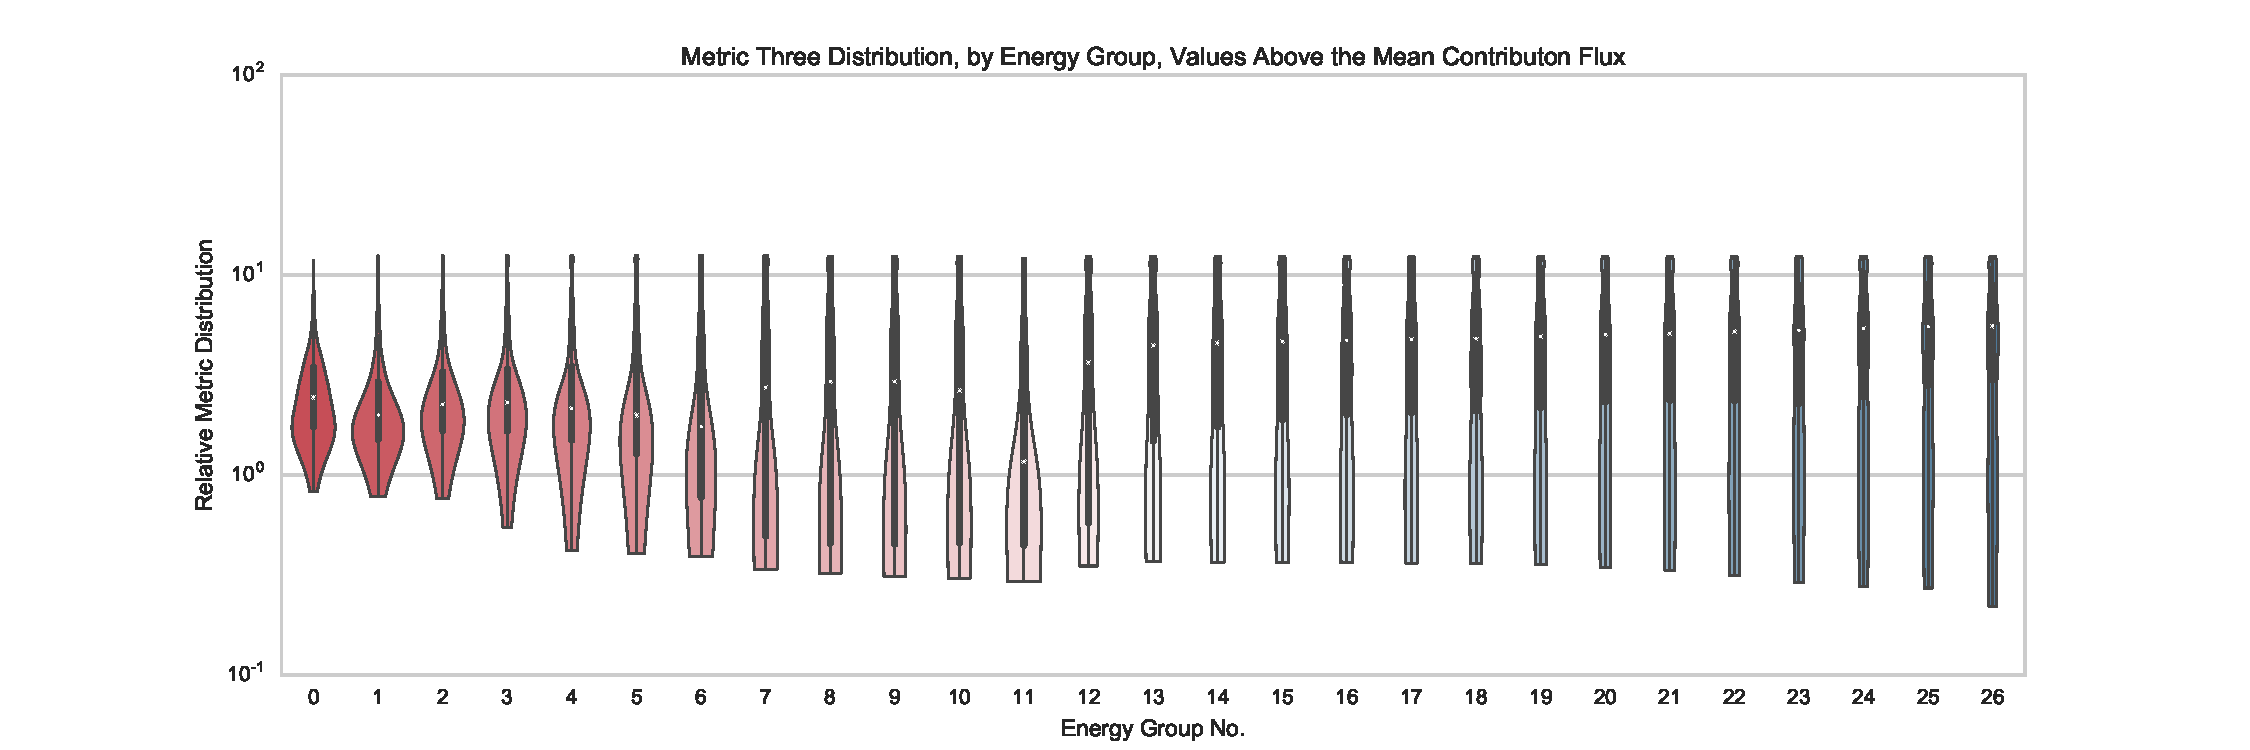
\includegraphics[width=\linewidth]{./chapters/characterization_probs/figures/char/maze1/metric_three_violin_mean.pdf}
    \caption{M$_3$ distribution for multi-turn labyrinth}
    \label{fig:maze1M3violins}
  \end{subfigure}
  \caption[Violin plots of M$_{3}$ distribution using values above the mean
  contributon flux for labyrinth problems.]
  {Violin plots of M$_{3}$ distribution using values above the mean
  contributon flux for labyrinth problems.}
  \label{fig:labyrinthviolins}
\end{figure}


\subsection{Steel Beam}
\label{subsec:resultbeam}

The steel beam embedded in concrete FOM and timing
results are summarized in Tables
\ref{tab:steelbeamfoms} and \ref{tab:steelbeamtimes}. Figures
\ref{fig:steelbeamresult} and \ref{fig:steelbeamerror} show the results obtained
by the track length tally in CADIS, CADIS-$\Omega$ and the nonbiased analog
Monte Carlo.

\begin{table}[h!]
  \centering
  \begin{tabular}{lrrrrr}
\toprule
{} &    cadis &             & cadisangle &             & analog \\
{} &       MC & MC\_adjusted &         MC & MC\_adjusted &     MC \\
\midrule
tally avg   &      668 &         659 &      3e+03 &    2.96e+03 &   1.39 \\
max RE      &     3.74 &        3.69 &       6.79 &        6.71 & 0.0448 \\
min RE      & 1.43e+03 &    1.41e+03 &   1.33e+03 &    1.31e+03 &    -- \\
time (mins) &      414 &         420 &   2.09e+03 &    2.11e+03 &   22.3 \\
\bottomrule
\end{tabular}

  \caption[Figure of Merit comparison for steel bar embedded in concrete.]
  {Figure of Merit comparison for steel bar embedded in concrete. }
  \label{tab:steelbeamfoms}
\end{table}

\begin{table}[h!]
  \centering
  \begin{tabular}{llrrr}
\toprule
          &             &          CADIS & CADIS-$\Omega$ &         analog \\
        &              & \multicolumn{3}{c}{time (minutes)} \\
\midrule
MCNP time & total &         414.45 &        2086.60 &          22.33 \\
deterministic time & advantg\_time &           0.18 &           0.18 &            -- \\
          & denovo\_time &           5.69 &          25.64 &            -- \\
          & dispose\_time &           0.00 &           0.16 &            -- \\
          & omega\_time &           0.00 &           0.66 &            -- \\
          & total &           5.87 &          26.49 &            -- \\
wall time &              &         420.32 &        2113.09 &          22.33 \\
\bottomrule
\end{tabular}

  \caption[Detailed timing results for steel bar embedded in concrete.]
  {Detailed timing results for steel bar embedded in concrete.}
  \label{tab:steelbeamtimes}
\end{table}

In the inspection of Tables \ref{tab:steelbeamfoms} and
\ref{tab:steelbeamtimes} we can conclude that this problem is very difficult for
analog Monte Carlo and that CADIS-$\Omega$ generally performs better than CADIS.
In fact, CADIS-$\Omega$ has the best performance
in this problem of all of the characterization problems.
CADIS-$\Omega$ outperforms CADIS for
the FOMS calculated with the tally average relative error and the tally maxmimum
relative error. This indicates that giving a limiting relative error to which
all energy bins must converge, CADIS-$\Omega$ will achieve it in half the time
that CADIS will. Further, CADIS-$\Omega$ has a better FOM than CADIS when the
deterministic runtimes are added. As shown in the timing table, the time to run
and generate the variance reduction parameters for CADIS-$\Omega$ will always be
longer than CADIS due to the forward transport run. The addition of
deterministic runtimes will always lower the FOM of CADIS-$\Omega$ more than
that of CADIS, so CADIS-$\Omega$'s achievement of a FOM higher FOM with much
longer runtimes in both Monte Carlo and ADVANTG illustrates just how much lower
the relative error it achieves is. CADIS-$\Omega$ is very well-suited to a
problem with these conditions.

\begin{figure}[h!]
  \centering
  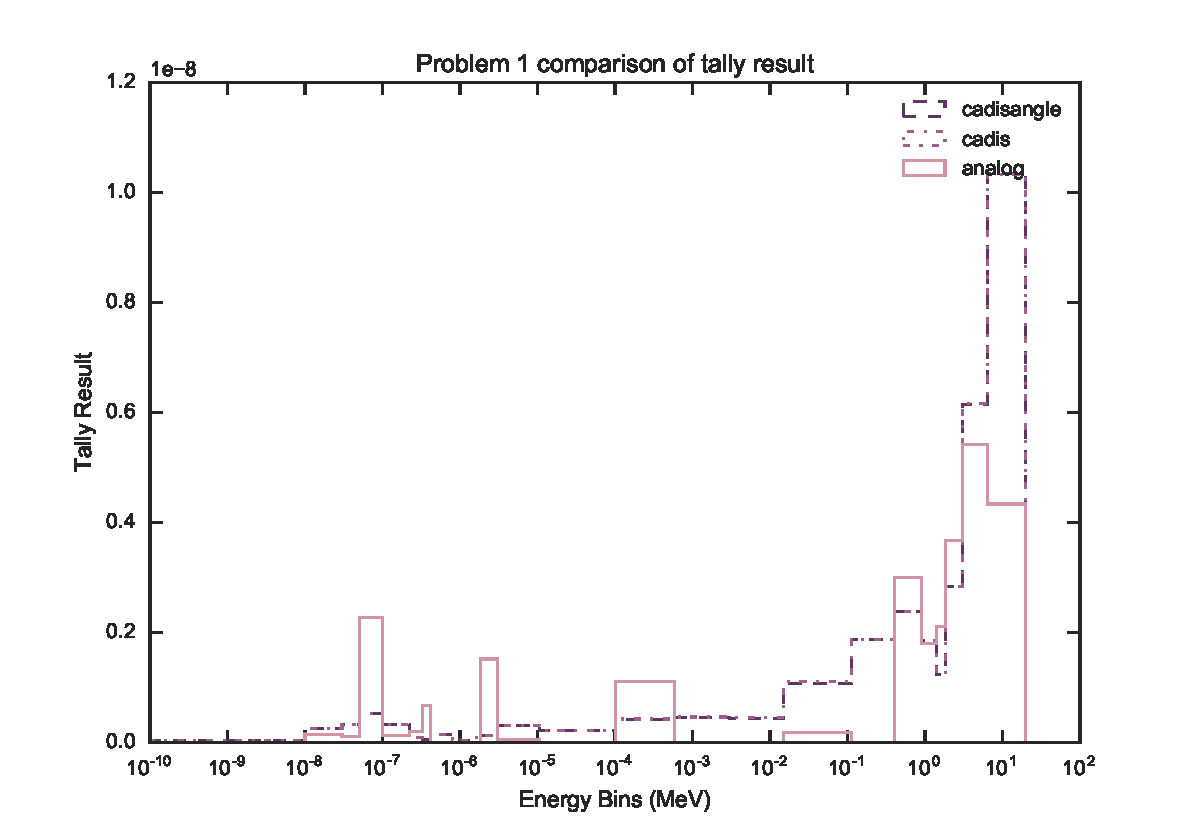
\includegraphics[height=10cm]{./chapters/characterization_probs/figures/char/prob_1/problem_1_tally_result_compare.pdf}
  \caption[Tally results comparison between methods for steel bar embedded in
  concrete.]
  {Tally results comparison between methods for steel bar embedded in concrete.}
  \label{fig:steelbeamresult}
\end{figure}

\begin{figure}[h!]
  \centering
  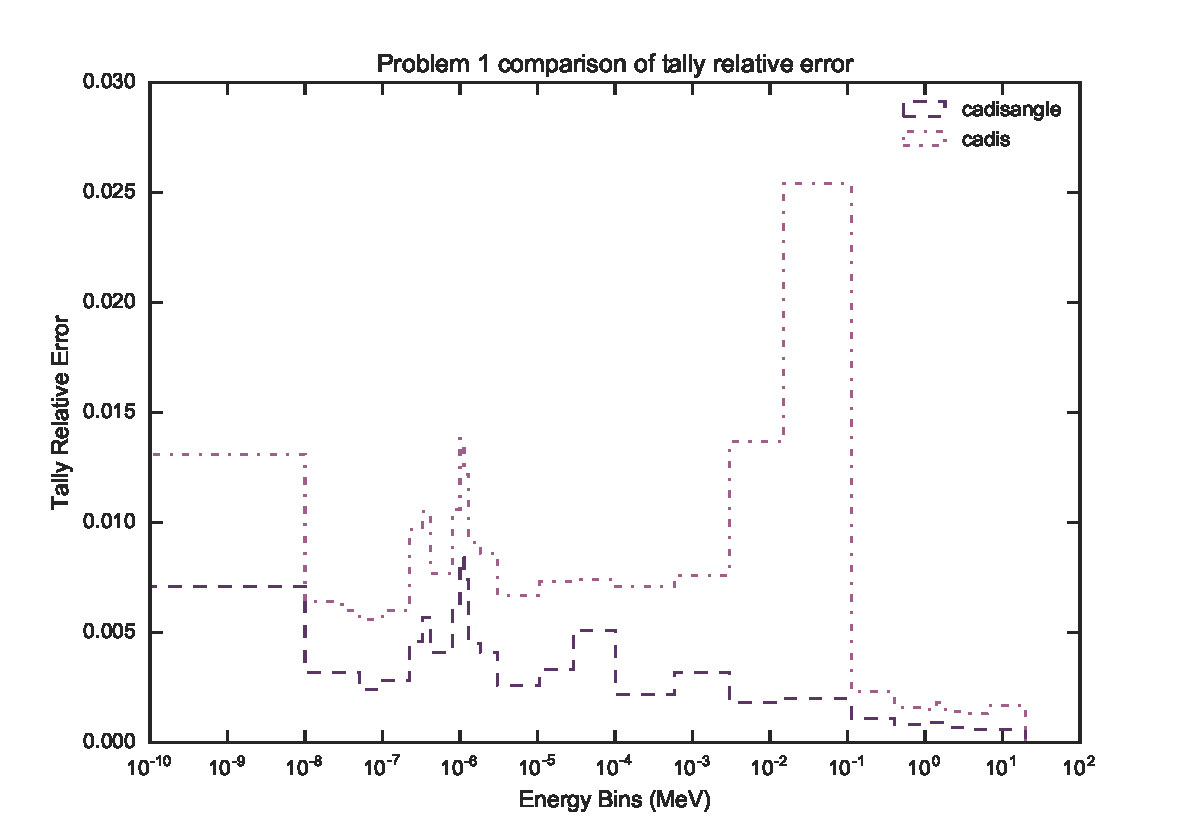
\includegraphics[height=10cm]{./chapters/characterization_probs/figures/char/prob_1/problem_1_tally_error_compare.pdf}
  \caption[Tally relative error comparison between methods for steel bar
  embedded in concrete.]
  {Tally relative error comparison between methods for steel bar embedded in
  concrete.}
  \label{fig:steelbeamerror}
\end{figure}

Figure \ref{fig:steelbeamresult} shows that CADIS and CADIS-$\Omega$ are in
agreement for the tally results in all energy bins. The nonbiased Monte Carlo
calculation differs from both of the hybrid methods. In Figure
\ref{fig:steelbeamerror} it can be observed that CADIS-$\Omega$ achieves a
consistently lower relative error than CADIS. From this we can conclude that
CADIS-$\Omega$'s source biasing parameters consistently move more particles in
all tally energy bins than CADIS. The importance map generated by CADIS-$\Omega$
better reflects the problem physics and more efficiently transports particles to
the desired tally location.

\subsubsection{Air Channel Variant}
\label{subsubsec:airbeam}

\begin{table}[h!]
  \centering
  \begin{tabular}{lrrrrr}
\toprule
{} & cadis &             & cadisangle &             & analog \\
{} &    MC & MC\_adjusted &         MC & MC\_adjusted &     MC \\
\midrule
tally avg   &   432 &         390 &        396 &         364 &   5.63 \\
max RE      &  1.17 &        1.05 &      0.247 &       0.227 & 0.0467 \\
min RE      &   273 &         247 &        296 &         272 &    -- \\
time (mins) &  47.3 &        52.3 &        247 &         268 &   21.4 \\
\bottomrule
\end{tabular}

  \caption[Figure of Merit comparison for steel bar geometry air variant.]
  {Figure of Merit comparison for steel bar geometry air variant. In this
  variant problem, the steel bar volume region is replaced with air to
exacerbate the suggested splitting issues encountered in other hybrid problems. }
  \label{tab:airbeamfoms}
\end{table}

\begin{table}[h!]
  \centering
  \begin{tabular}{llrrr}
\toprule
          &              &          cadis &     cadisangle &         analog \\
          &              & time (minutes) & time (minutes) & time (minutes) \\
\midrule
MCNP time & total &          47.29 &         246.83 &          21.42 \\
deterministic time & advantg\_time &           0.16 &           0.15 &            -- \\
          & denovo\_time &           4.90 &          20.50 &            -- \\
          & dispose\_time &           0.00 &           0.15 &            -- \\
          & omega\_time &           0.00 &           0.65 &            -- \\
          & total &           5.05 &          21.30 &            -- \\
wall time &              &          52.34 &         268.13 &          21.42 \\
\bottomrule
\end{tabular}

  \caption[Detailed timing results for steel bar geometry air variant.]
  {Detailed timing results for steel bar geometry air variant.}
  \label{tab:airbeamtimes}
\end{table}

\subsubsection{Concrete Channel Variant}
\label{subsubsec:concretebeam}

\begin{table}[h!]
  \centering
  \begin{tabular}{lrrrrr}
\toprule
{} &    cadis &             & cadisangle &             & analog \\
{} &       MC & MC\_adjusted &         MC & MC\_adjusted &     MC \\
\midrule
tally avg   &  2.6e+03 &    2.55e+03 &   3.16e+03 &    3.13e+03 &   1.54 \\
max RE      &     14.5 &        14.2 &       9.48 &        9.39 & 0.0457 \\
min RE      & 1.54e+03 &    1.51e+03 &    1.4e+03 &    1.39e+03 &    -- \\
time (mins) &      385 &         393 &   1.98e+03 &       2e+03 &   21.9 \\
\bottomrule
\end{tabular}

  \caption[Figure of Merit comparison for steel bar geometry concrete variant.]
  {Figure of Merit comparison for steel bar geometry concrete variant. In this
  variant problem, the steel bar volume region is replaced with concrete to
  eliminate the preferential particle travel through the beam region. This
  should reduce the angular dependence in the problem, but not have splitting
  issues like the air channel. }
  \label{tab:airbeamfoms}
\end{table}

\begin{table}[h!]
  \centering
  \begin{tabular}{llrrr}
\toprule
          &              &          cadis &     cadisangle &         analog \\
          &              & time (minutes) & time (minutes) & time (minutes) \\
\midrule
MCNP time & total &         385.11 &        1978.46 &          21.88 \\
deterministic time & advantg\_time &           0.23 &           0.15 &            -- \\
          & denovo\_time &           7.42 &          19.58 &            -- \\
          & dispose\_time &           0.00 &           0.09 &            -- \\
          & omega\_time &           0.00 &           0.56 &            -- \\
          & total &           7.65 &          20.29 &            -- \\
wall time &              &         392.76 &        1998.75 &          21.88 \\
\bottomrule
\end{tabular}

  \caption[Detailed timing results for steel bar geometry air variant.]
  {Detailed timing results for steel bar geometry air variant.}
  \label{tab:airbeamtimes}
\end{table}

\subsection{U-Shaped Corridor}
\label{subsec:resultsucorridor}

The U-shaped air corridor embedded in concrete
FOM and timing
results are summarized in Tables
\ref{tab:ucorridorfoms} and \ref{tab:ucorridortimes}. Figures
\ref{fig:ucorridorresult} and \ref{fig:ucorridorerror} show the results obtained
by the track length tally in CADIS, CADIS-$\Omega$ and the nonbiased analog
Monte Carlo.

\begin{table}[h!]
  \centering
  \begin{tabular}{lrrrrr}
\toprule
{} &  cadis &             & cadisangle &             & analog \\
{} &     MC & MC\_adjusted &         MC & MC\_adjusted &     MC \\
\midrule
tally avg   &   64.1 &        51.9 &       60.2 &        38.3 &  0.378 \\
max RE      & 0.0183 &      0.0148 &     0.0144 &     0.00913 & 0.0644 \\
min RE      &   14.9 &          12 &       13.4 &        8.54 &    -- \\
time (mins) &   54.6 &        67.5 &        188 &         296 &   15.5 \\
\bottomrule
\end{tabular}

  \caption[Figure of Merit comparison between methods for U-shaped air corridor in concrete.]
  {Figure of Merit comparison between methods for U-shaped air corridor in
  concrete.}
  \label{tab:ucorridorfoms}
\end{table}

\begin{table}[h!]
  \centering
  \begin{tabular}{llrrr}
\toprule
          &             &          CADIS & CADIS-$\Omega$ &         analog \\
        &              & \multicolumn{3}{c}{time (minutes)} \\
\midrule
MCNP time & total &          54.61 &         187.92 &          15.54 \\
deterministic time & advantg\_time &           0.19 &           0.21 &            -- \\
          & denovo\_time &          12.68 &         105.90 &            -- \\
          & dispose\_time &           0.01 &           0.35 &            -- \\
          & omega\_time &           0.00 &           1.49 &            -- \\
          & total &          12.87 &         107.60 &            -- \\
wall time &              &          67.48 &         295.52 &          15.54 \\
\bottomrule
\end{tabular}

  \caption[Detailed timing results for U-shaped air corridor in concrete.]
  {Detailed timing results for U-shaped air corridor in concrete.}
  \label{tab:ucorridortimes}
\end{table}

\begin{figure}[h!]
  \centering
  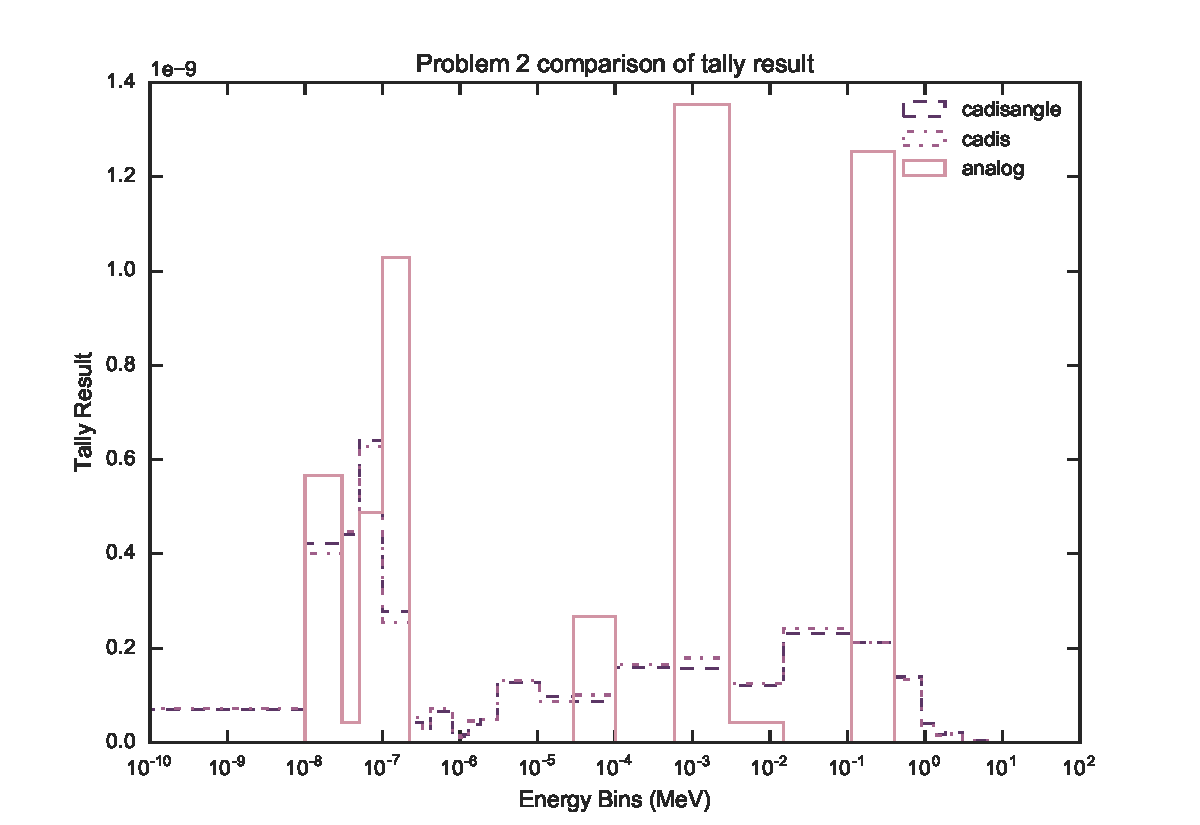
\includegraphics[height=10cm]{./chapters/characterization_probs/figures/char/prob_2/problem_2_tally_result_compare.pdf}
  \caption[Tally results comparison between methods for U-shaped air corridor in
  concrete.]
  {Tally results comparison between methods for U-shaped air corridor in
  concrete.}
  \label{fig:ucorridorresult}
\end{figure}

\begin{figure}[h!]
  \centering
  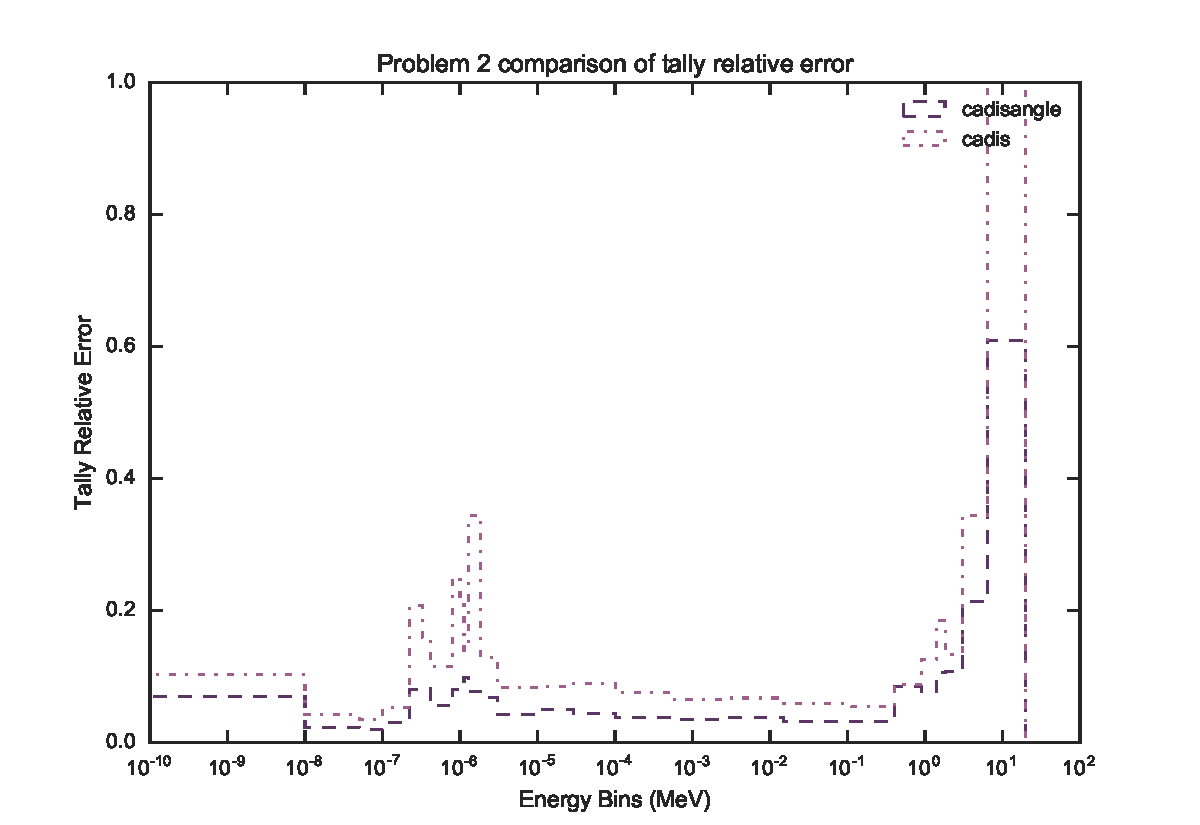
\includegraphics[height=10cm]{./chapters/characterization_probs/figures/char/prob_2/problem_2_tally_error_compare.pdf}
  \caption[Tally relative error comparison between methods for U-shaped air
  corridor in concrete.]
  {Tally relative error comparison between methods for U-shaped air corridor in
  concrete.}
  \label{fig:ucorridorerror}
\end{figure}
% [Table of FOMs for this problem] \\
%
% [Plot of tally results for this problem] \\
%
% [Plot of anisotropies for this problem] \\
%
% [Summarize results and describe issues affecting performance] \\

\subsection{Shielding with Rebar}
\label{subsec:resultrebar}

The problem with rebar embedded length- and width-wise
in concrete has FOM and timing
results summarized in Tables
\ref{tab:rebarfoms} and \ref{tab:rebartimes}. Figures
\ref{fig:rebarresult} and \ref{fig:rebarerror} show the results obtained
by the track length tally in CADIS, CADIS-$\Omega$ and the nonbiased analog
Monte Carlo.

\begin{table}[h!]
  \centering
  \begin{tabular}{lrrrrr}
\toprule
{} & \multicolumn{2}{c}{CADIS}   & \multicolumn{2}{c}{CADIS-$\Omega$}  & analog \\
{} &    MC & MC$_{hybrid}$ &         MC & MC$_{hybrid}$ &     MC \\
\midrule
tally avg   &   1.15 &        1.09 &     0.0136 &      0.0127 &  0.948 \\
max RE      & 0.0345 &      0.0327 &    0.00117 &     0.00109 & 0.0186 \\
min RE      &    235 &         223 &        199 &         186 &    -- \\
time (mins) &    328 &         346 &   1.55e+03 &    1.66e+03 &   53.8 \\
\bottomrule
\end{tabular}

  \caption[Figure of Merit comparison between methods for rebar-embedded
  concrete.]{Figure of Merit comparison between methods for rebar-embedded
  concrete.}
  \label{tab:rebarfoms}
\end{table}

\begin{table}[h!]
  \centering
  \begin{tabular}{llrrr}
\toprule
          &              &          cadis &     cadisangle &         analog \\
          &              & time (minutes) & time (minutes) & time (minutes) \\
\midrule
MCNP time & total &         327.81 &        1550.54 &          53.82 \\
deterministic time & advantg\_time &           0.28 &           0.29 &            -- \\
          & denovo\_time &          17.70 &         105.09 &            -- \\
          & dispose\_time &           0.03 &           0.41 &            -- \\
          & omega\_time &           0.00 &           2.05 &            -- \\
          & total &          17.98 &         107.43 &            -- \\
wall time &              &         345.79 &        1657.97 &          53.82 \\
\bottomrule
\end{tabular}

  \caption[Detailed timing results for rebar-embedded concrete]
  {Detailed timing results for rebar-embedded concrete.}
  \label{tab:rebartimes}
\end{table}

\begin{figure}[h!]
  \centering
  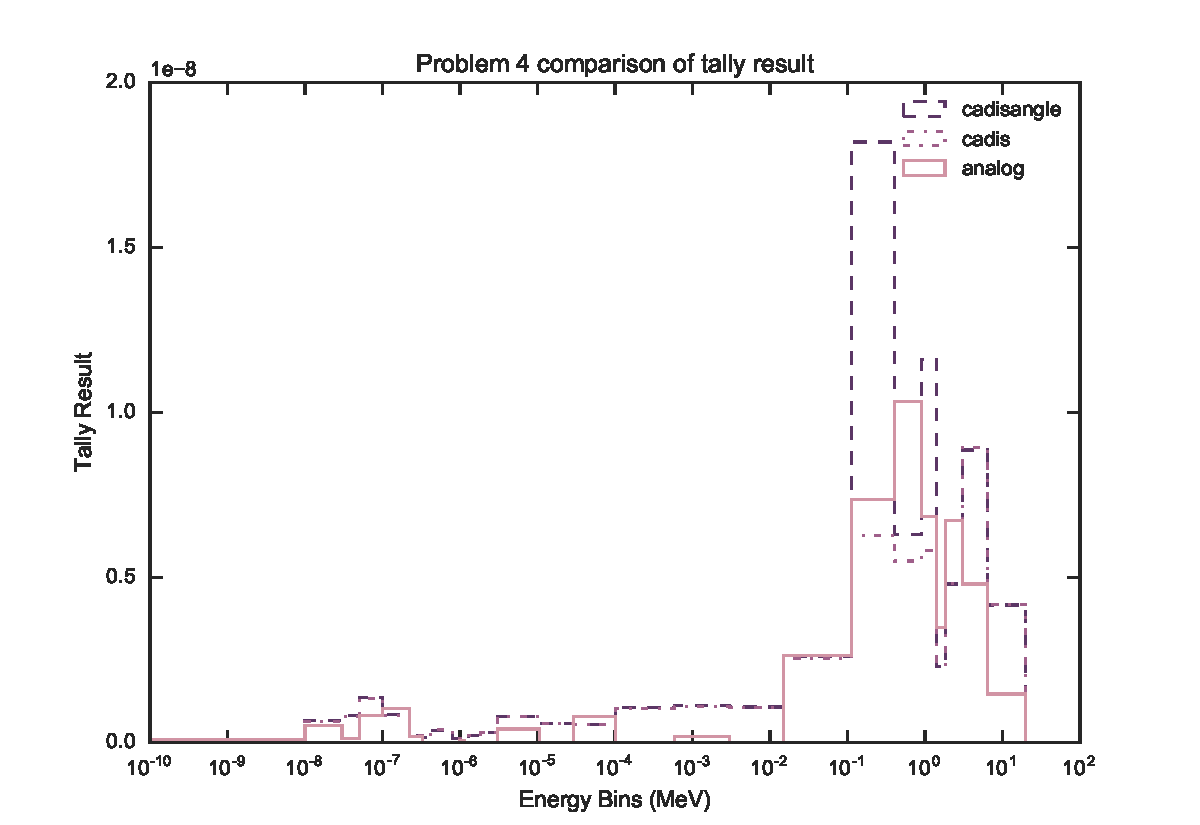
\includegraphics[height=10cm]{./chapters/characterization_probs/figures/char/prob_4/problem_4_tally_result_compare.pdf}
  \caption[Tally results comparison between methods for rebar-embedded concrete.]
  {Tally results comparison between methods for rebar-embedded concrete.}
  \label{fig:rebarresult}
\end{figure}

\begin{figure}[h!]
  \centering
  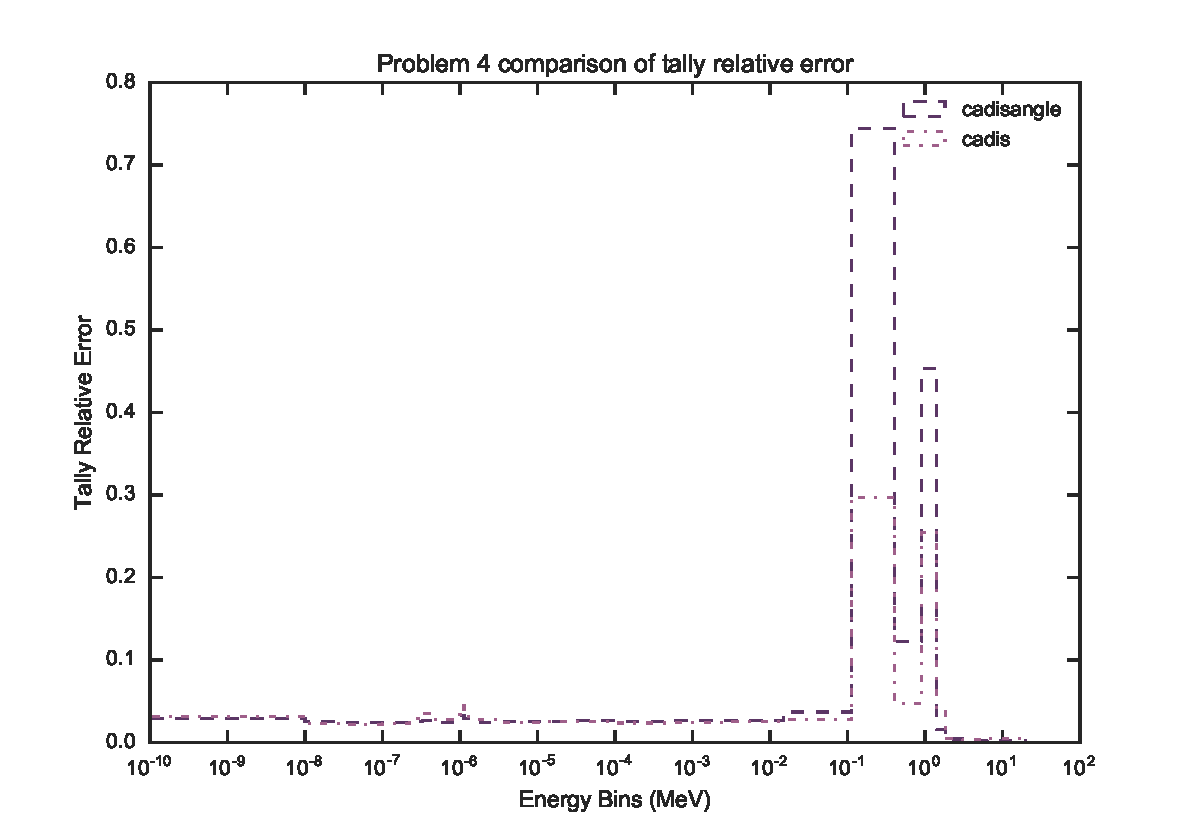
\includegraphics[height=10cm]{./chapters/characterization_probs/figures/char/prob_4/problem_4_tally_error_compare.pdf}
  \caption[Tally relative error comparison between methods for rebar-embedded concrete.]
  {Tally relative error comparison between methods for rebar-embedded concrete.}
  \label{fig:rebarerror}
\end{figure}
% [Table of FOMs for this problem] \\
%
% [Plot of tally results for this problem] \\
%
% [Plot of anisotropies for this problem] \\
%
% [Summarize results and describe issues affecting performance] \\

\subsection{Beam Problem}
\label{subsec:resultsbeam}

The nuclear physics beamline toy problem has FOM and timing
results summarized in Tables
\ref{tab:beamfoms} and \ref{tab:beamtimes}. Figures
\ref{fig:beamresult} and \ref{fig:beamerror} show the results obtained
by the track length tally in CADIS, CADIS-$\Omega$ and the nonbiased analog
Monte Carlo.

\begin{table}[h!]
  \centering
  \begin{tabular}{lrrrrr}
\toprule
{} & cadis &             & cadisangle &             & analog \\
{} &    MC & MC\_adjusted &         MC & MC\_adjusted &     MC \\
\midrule
tally avg   &   368 &         138 &       94.8 &        7.91 &    317 \\
max RE      & 0.542 &       0.202 &       1.18 &      0.0984 &    1.6 \\
min RE      &   -- &         -- &        -- &         -- &    -- \\
time (mins) &  2.23 &        5.97 &       1.69 &        20.3 &   1.69 \\
\bottomrule
\end{tabular}

  \caption[Figure of Merit comparison between methods for simplified
    experimental nuclear physics beamline.]
    {Figure of Merit comparison between methods for simplified experimental
    nuclear physics beamline.}
  \label{tab:beamfoms}
\end{table}

\begin{table}[h!]
  \centering
  \begin{tabular}{llrrr}
\toprule
          &             &          CADIS & CADIS-$\Omega$ &         analog \\
        &              & \multicolumn{3}{c}{time (minutes)} \\
\midrule
MCNP time & total &           2.23 &           1.69 &           1.69 \\
deterministic time & advantg\_time &           0.17 &           0.15 &            -- \\
          & denovo\_time &           3.57 &          17.88 &            -- \\
          & dispose\_time &           0.00 &           0.12 &            -- \\
          & omega\_time &           0.00 &           0.53 &            -- \\
          & total &           3.74 &          18.56 &            -- \\
wall time &              &           5.97 &          20.25 &           1.69 \\
\bottomrule
\end{tabular}

  \caption[Detailed timing results for simplified experimental nuclear physics
  beamline.]
  {Detailed timing results for simplified experimental nuclear physics beamline.}
  \label{tab:steelbeamtimes}
\end{table}

\begin{figure}[h!]
  \centering
  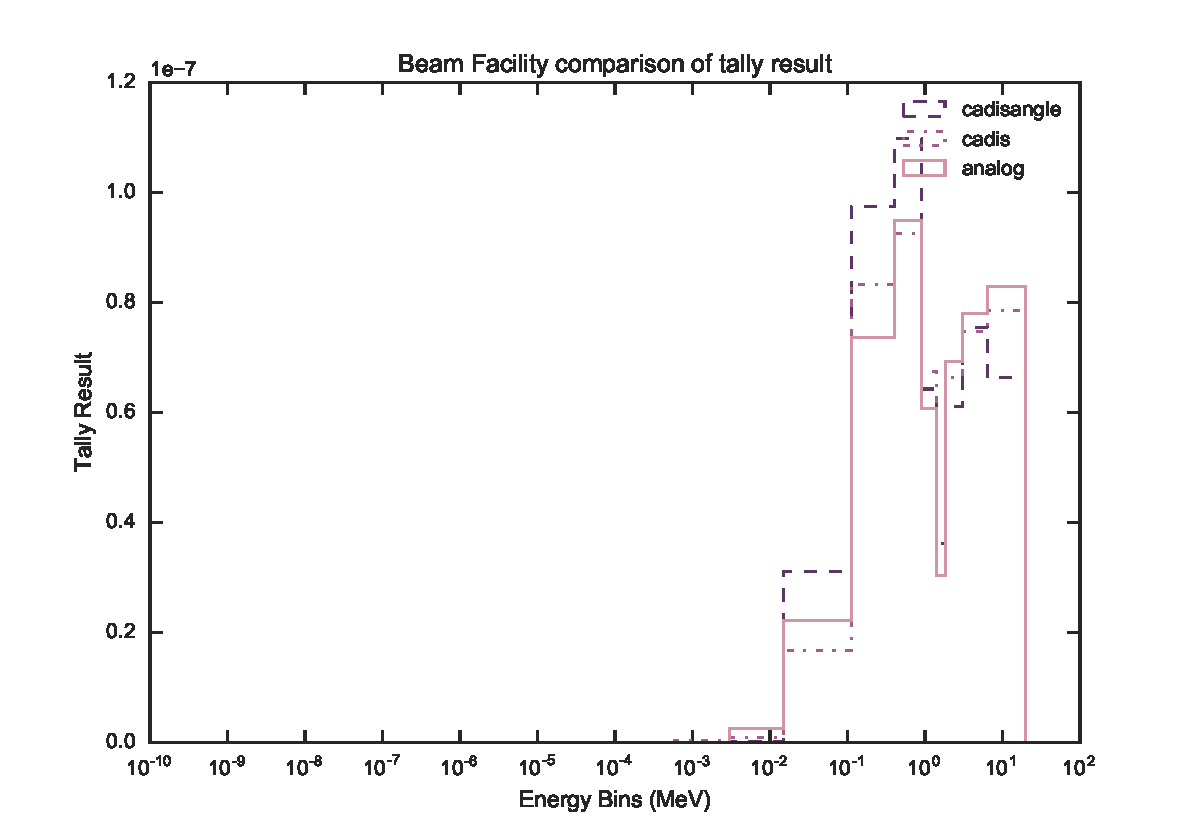
\includegraphics[height=10cm]{./chapters/characterization_probs/figures/char/beam/beam_facility_tally_result_compare.pdf}
  \caption[Tally results comparison between methods for simplified experimental
    nuclear physics beamline.]
  {Tally results comparison between methods for simplified experimental
    nuclear physics beamline.}
  \label{fig:beamresult}
\end{figure}

\begin{figure}[h!]
  \centering
  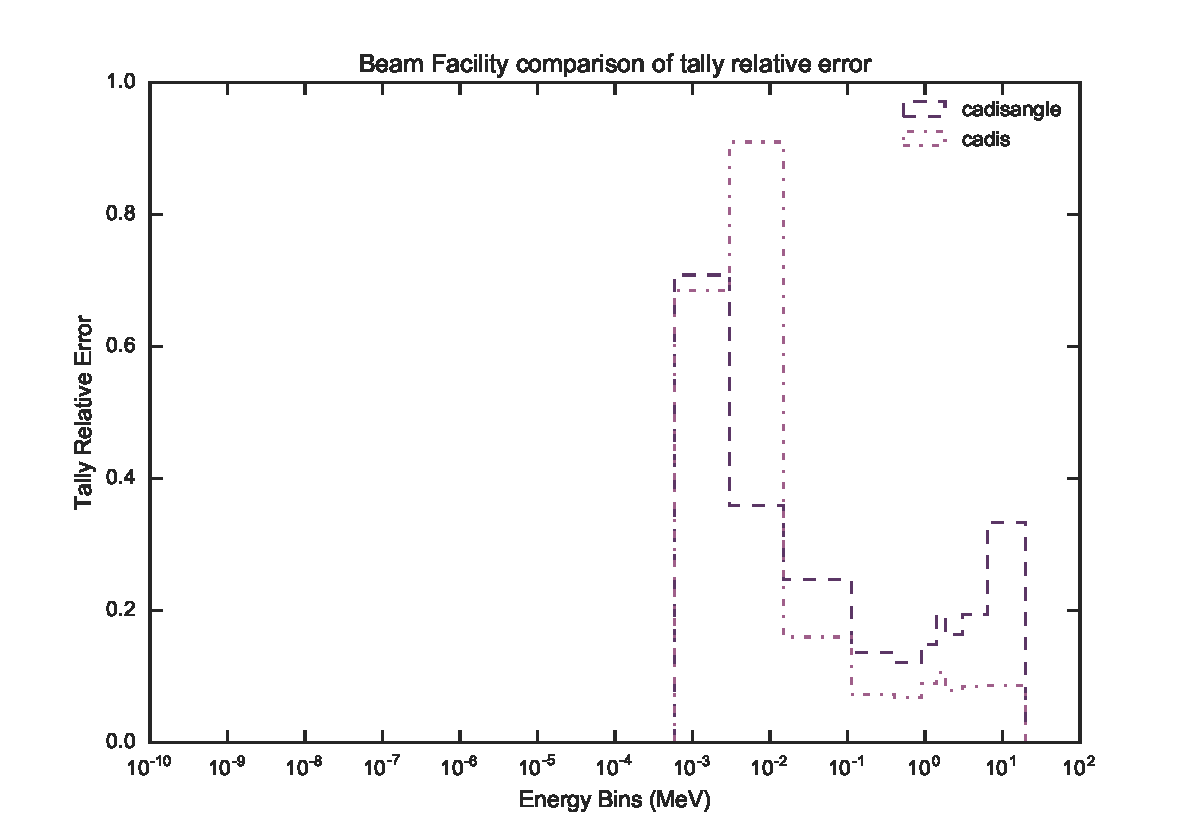
\includegraphics[height=10cm]{./chapters/characterization_probs/figures/char/beam/beam_facility_tally_error_compare.pdf}
  \caption[Tally relative error comparison between methods
    for simplified experimental nuclear physics beamline.]
  {Tally relative error comparison between methods for simplified experimental
    nuclear physics beamline.}
  \label{fig:beamerror}
\end{figure}
% [Table of FOMs for this problem] \\
%
% [Plot of tally results for this problem] \\
%
% [Plot of anisotropies for this problem] \\
%
% [Summarize results and describe issues affecting performance] \\

\subsection{Therapy Room}
% \label{subsec:resultstherapy}
% \begin{table}[h!]
%   \centering
%   \input{./chapters/characterization_probs/figures//_tally_foms_compare}
%   \caption[]{}
%   \label{tab:foms}
% \end{table}

% \begin{figure}[h!]
%   \centering
%   \includegraphics[height=10cm]{./chapters/characterization_probs/figures/char/_tally_result_compare.pdf}
%   \caption[Tally results comparison between methods for ]
%   {Tally results comparison between methods for }
%   \label{fig:result}
% \end{figure}

% \begin{figure}[h!]
%   \centering
%   \includegraphics[height=10cm]{./chapters/characterization_probs/figures/char/_tally_error_compare.pdf}
%   \caption[Tally relative error comparison between methods for ]
%   {Tally relative error comparison between methods for}
%   \label{fig:result}
% \end{figure}
% [Table of FOMs for this problem] \\
%
% [Plot of tally results for this problem] \\
%
% [Plot of anisotropies for this problem] \\
%
% [Summarize results and describe issues affecting performance] \\

